% Standalone figure for the Statistical Mechanics notes.
% Build: pdflatex unary-fv.tex  (or run build.sh in this folder)
\documentclass[11pt,tikz,border=2pt]{standalone}
\usepackage{amsmath,amssymb}
\usetikzlibrary{arrows.meta, positioning}
\begin{document}
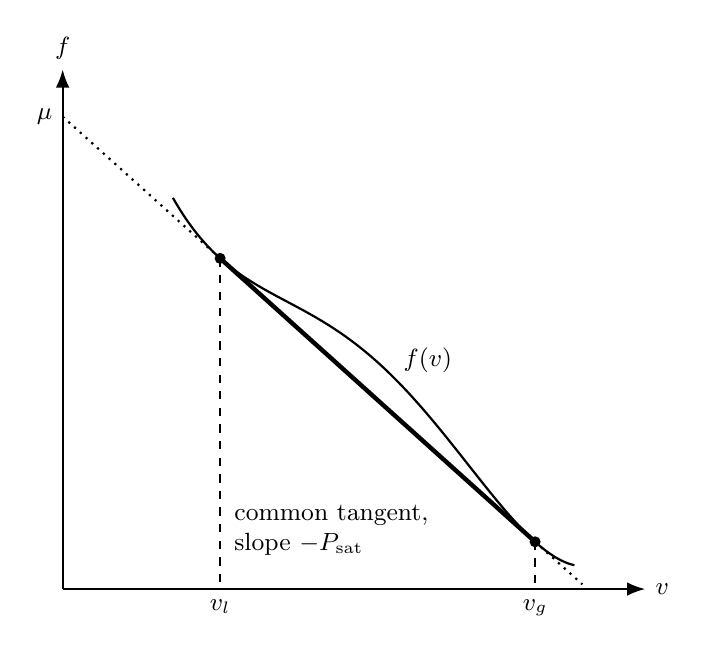
\begin{tikzpicture}[font=\small, >=Latex, line width=0.8pt]
    % axes
    \draw[->] (0,0) -- (7.4,0) node[right] {$v$};
    \draw[->] (0,0) -- (0,6.6) node[above] {$f$};
    % single-phase curve f(v) = tangent + 0.05 (v-2)^2 (v-6)^2, scaled by 0.6
    \draw[domain=1.4:6.5, smooth, variable=\t, samples=60]
        plot ({\t},{0.6*(10-1.5*\t+0.05*(\t-2)^2*(\t-6)^2)});
    % common tangent, extended to v = 0 to show the intercept mu
    \draw[dotted] (0,6) -- (2,4.2);
    \draw[line width=1.6pt] (2,4.2) -- (6,0.6);
    \draw[dotted] (6,0.6) -- (6.6,0.06);
    % tangent points
    \fill (2,4.2) circle (2pt);
    \fill (6,0.6) circle (2pt);
    \draw[dashed] (2,4.2) -- (2,0) node[below] {$v_l$};
    \draw[dashed] (6,0.6) -- (6,0) node[below] {$v_g$};
    % intercept
    \node[left] at (0,6) {$\mu$};
    % labels
    \node[right] at (4.2,2.9) {$f(v)$};
    \node[align=left, right] at (2.05,0.75) {common tangent,\\ slope $-P_{\text{sat}}$};
\end{tikzpicture}
\end{document}
